\documentclass[12pt,a4paper]{article}

\usepackage[T1]{fontenc}
\usepackage[utf8]{inputenc}
\usepackage[polish]{babel}
\usepackage{indentfirst}
\usepackage{amsfonts}
\usepackage{amsmath}
\usepackage{algorithmic}

\usepackage[margin=0.5in,headheight=48pt,top=78pt]{geometry}
\frenchspacing
\setlength{\parskip}{1em}
\setlength{\parindent}{0em}
\def\N{\mathbb{N}}
\def\R{\mathbb{R}}
\newcommand{\zadanie}[1]{\par\textbf{Zadanie #1}}
\newcommand{\odp}[1]{\textbf{Odpowiedź:} #1}


\usepackage{tikz}

\usepackage{fancyhdr}
\pagestyle{fancy}
\fancyhf{} % clear all fields
\fancyhead[C]{ \textbf{AISD} - Lista 4 Zadanie 8\ Wiktor Pilarczyk 308533}

\begin{document}
\section{Wprowadzenie}
Na szachownicy z 4 x n polami, do których jest przypisane są liczby naturalne chcemy poukładać kamienie tak, żeby zmaksymalizować sumę liczb na zajętych polach. Nie chcemy, żeby dwa kamienie ze sobą sąsiadowały (pola ze wspólną krawędzią) oraz na jednym polu może być tylko jeden kamyk.

Łatwo zauważyć, że mamy 8 możliwości ustawienia kamyków w jednej kolumnie.

\begin{figure}[!htb]
\centering
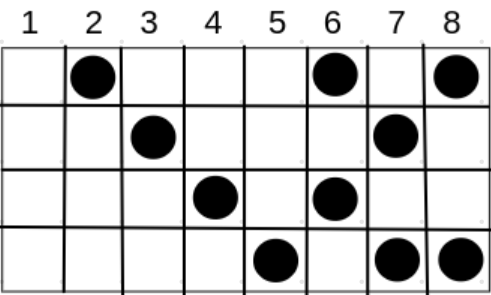
\includegraphics[scale=0.45]{mozliwosci.png}
\caption{Wszystkie możliwości}
\end{figure}

Możliwość ustawienia kamyków w jednej kolumnie jest zależne od sąsiednich kolumn.
\section{Algorytm}
Nasz algorytm będzie dynamikiem, gdzie problem sprowadzamy do szachownicy o mniejszej liczbie kolumn i mając wcześniej obliczone maksymalne wartości jakie możemy uzyskać dla k-tej kolumny (dla każdej możliwości ułożenia ostatniej kolumny) to jesteśmy w stanie obliczyć wyniki dla k+1 kolumny.

\begin{figure}[!htb]
\centering
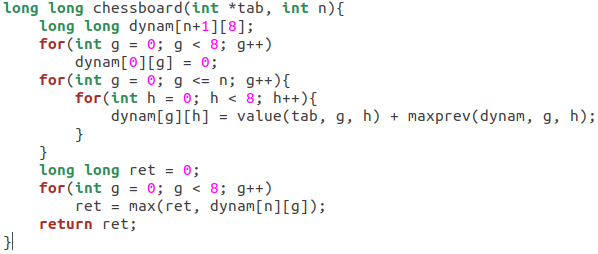
\includegraphics[scale=0.7]{algo2.png}
\caption{Pseudokod algorytmu}
\end{figure}

Funkcja value oblicza wartość ułożenia kamyków w g-tej kolumnie dla h-tego sposobu, zaś funkcja maxprev zwraca maksymalną wartość jaką mogła mieć g-1 kolumna, która może sąsiadować z h-tym sposobem ułożenia kamyków.
Pod koniec zwracamy maksimum z obliczonych wartości dla każdej możliwości ustawienia ostatniej kolumny.

Szukana wartość jest maksimum z sposobów ułożenia dla ostatniej kolumny.
\section{Dowód poprawności}
Dowód będzie indukcyjny względem k-tej kolumny.

Teza indukcji: dla k-tej kolumny mamy obliczone największe wartości, które można otrzymać dla każdego sposobu ułożenia kolumny.

Baza indukcji:

k = 1
wtedy obliczamy tylko wartość dla każdej kolumny, ponieważ maxprev zwróci zero.

Krok indukcyjny:

Założenie indukcyjne: teza jest spełniona dla k-tej kolumny
Teza indukcyjna: teza jest spełniona dla k+1. kolumny

Wiemy, że maksymalna wartość dla k+1. kolumny i h-tego sposobu, jest to suma wartości kamyków z tej kolumny oraz maksymalna wartość jaką mogliśmy otrzymać wcześniej, czyli maksymalna wartość dla k-tej kolumny z ułożeniem, które nie koliduje z naszym, a ponieważ z założenia indukcyjnego mamy już te możliwości dla k obliczone to możemy je obliczyć też dla k+1.

\section{Złożoność}
Wyliczenie wartości dla każdej kolumny jest wykonane w czasie stałym (mamy ograniczoną liczbe możliwość i ograniczoną liczbe możliwych sąsiadów), a ponieważ musimy wykonać obliczenia dla każdej kolumny to złożoność naszego algorytmu wynosi $\Theta(n)$.

\end{document}

